\section{Design Pattern 2}

\subsection{Description Design Pattern 2}
The definition of our levels are made in a .txt file. The problem here is determining what object of Model is loaded where. In the Factory Method pattern this is fixed by a Factory. In our case it's called LevelFactory. LevelController calls this class to load the .txt file, and eventually create all objects that are noted in the file. Then it returns a Level which LevelController uses.


\subsection{Class Diagram Design Pattern 2}

Below is the class diagram of the Factory design pattern, found as in our code.
\\\\
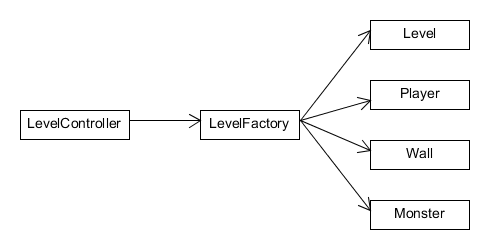
\includegraphics[width=100mm]{UML_factory.png}

\subsection{Sequence Diagram Design Pattern 2}

Below is the sequence diagram of the Factory design pattern, as found in our code.
\\\\
\includegraphics[width=150mm]{factory_sequence.jpg}